
\documentclass[a4paper, landscape]{article}
\usepackage{pgfplots}
\pgfplotsset{small,  compat=1.5}
\begin{document}

\pgfplotsset{
small
}


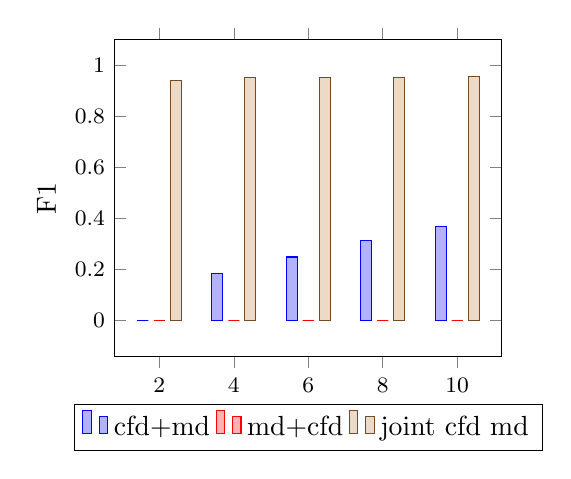
\begin{tikzpicture} \begin{axis}[
ybar,
enlargelimits=0.15,
legend style={at={(0.5,-0.15)}, anchor=north,legend columns=-1},
bar width=4,
ylabel={F1},
symbolic x coords={2,4,6,8,10},
xtick=data,
nodes near coords align={vertical},
]
\addplot coordinates {(2, 0.0) (4, 0.184) (6, 0.2479) (8, 0.313) (10, 0.3676)};
\addplot coordinates {(2, 0.0) (4, 0.0) (6, 0.0) (8, 0.0) (10, 0.0)};
\addplot coordinates {(2, 0.9402) (4, 0.9511) (6, 0.9528) (8, 0.9534) (10, 0.9574)};

\legend{cfd+md,md+cfd,joint cfd md}
\end{axis}
\end{tikzpicture}
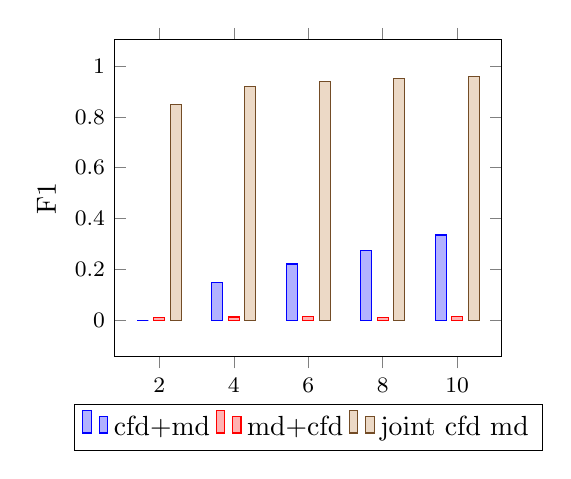
\begin{tikzpicture} \begin{axis}[
ybar,
enlargelimits=0.15,
legend style={at={(0.5,-0.15)}, anchor=north,legend columns=-1},
bar width=4,
ylabel={F1},
symbolic x coords={2,4,6,8,10},
xtick=data,
nodes near coords align={vertical},
]
\addplot coordinates {(2, 0.0) (4, 0.1479) (6, 0.221) (8, 0.2745) (10, 0.3351)};
\addplot coordinates {(2, 0.0094) (4, 0.0124) (6, 0.0133) (8, 0.0109) (10, 0.0127)};
\addplot coordinates {(2, 0.8502) (4, 0.9184) (6, 0.9396) (8, 0.9524) (10, 0.9601)};

\legend{cfd+md,md+cfd,joint cfd md}
\end{axis}
\end{tikzpicture}
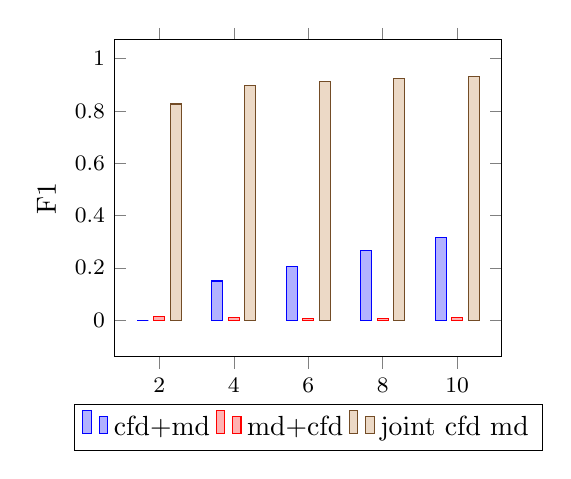
\begin{tikzpicture} \begin{axis}[
ybar,
enlargelimits=0.15,
legend style={at={(0.5,-0.15)}, anchor=north,legend columns=-1},
bar width=4,
ylabel={F1},
symbolic x coords={2,4,6,8,10},
xtick=data,
nodes near coords align={vertical},
]
\addplot coordinates {(2, 0.0) (4, 0.1494) (6, 0.205) (8, 0.2665) (10, 0.3146)};
\addplot coordinates {(2, 0.0122) (4, 0.0117) (6, 0.0063) (8, 0.0076) (10, 0.0084)};
\addplot coordinates {(2, 0.8261) (4, 0.8959) (6, 0.9109) (8, 0.9232) (10, 0.9321)};

\legend{cfd+md,md+cfd,joint cfd md}
\end{axis}
\end{tikzpicture}
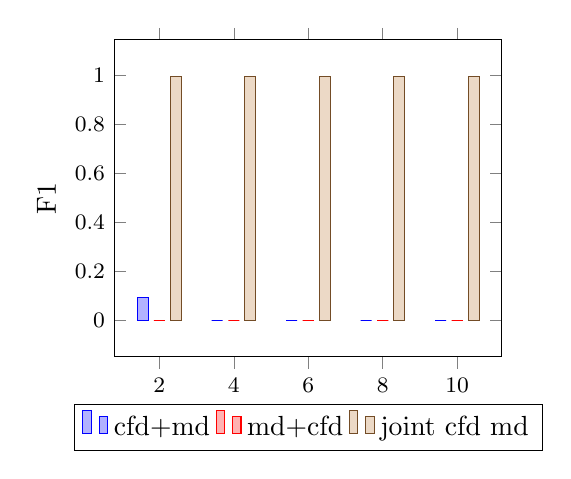
\begin{tikzpicture} \begin{axis}[
ybar,
enlargelimits=0.15,
legend style={at={(0.5,-0.15)}, anchor=north,legend columns=-1},
bar width=4,
ylabel={F1},
symbolic x coords={2,4,6,8,10},
xtick=data,
nodes near coords align={vertical},
]
\addplot coordinates {(2, 0.0907) (4, 0.0) (6, 0.0) (8, 0.0) (10, 0.0)};
\addplot coordinates {(2, 0.0) (4, 0.0) (6, 0.0) (8, 0.0) (10, 0.0)};
\addplot coordinates {(2, 0.9956) (4, 0.9934) (6, 0.9934) (8, 0.9939) (10, 0.9956)};

\legend{cfd+md,md+cfd,joint cfd md}
\end{axis}
\end{tikzpicture}
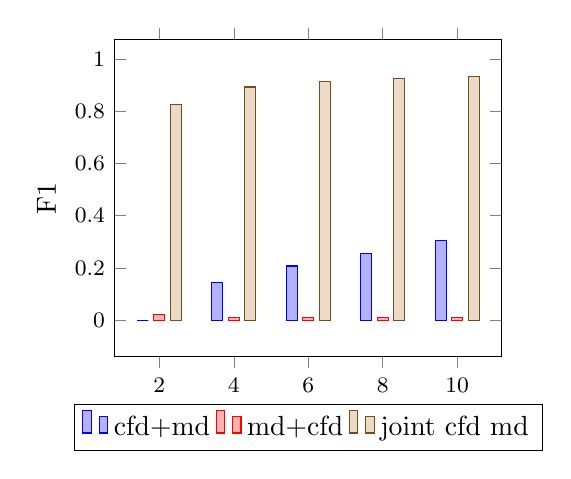
\begin{tikzpicture} \begin{axis}[
ybar,
enlargelimits=0.15,
legend style={at={(0.5,-0.15)}, anchor=north,legend columns=-1},
bar width=4,
ylabel={F1},
symbolic x coords={2,4,6,8,10},
xtick=data,
nodes near coords align={vertical},
]
\addplot coordinates {(2, 0.0) (4, 0.1447) (6, 0.2071) (8, 0.2566) (10, 0.3054)};
\addplot coordinates {(2, 0.0209) (4, 0.0115) (6, 0.0114) (8, 0.0105) (10, 0.01)};
\addplot coordinates {(2, 0.8272) (4, 0.8927) (6, 0.9131) (8, 0.926) (10, 0.9337)};

\legend{cfd+md,md+cfd,joint cfd md}
\end{axis}
\end{tikzpicture}
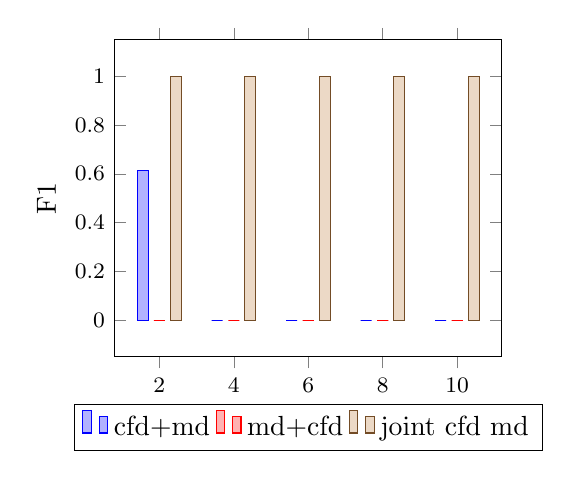
\begin{tikzpicture} \begin{axis}[
ybar,
enlargelimits=0.15,
legend style={at={(0.5,-0.15)}, anchor=north,legend columns=-1},
bar width=4,
ylabel={F1},
symbolic x coords={2,4,6,8,10},
xtick=data,
nodes near coords align={vertical},
]
\addplot coordinates {(2, 0.6154) (4, 0.0) (6, 0.0) (8, 0.0) (10, 0.0)};
\addplot coordinates {(2, 0.0) (4, 0.0) (6, 0.0) (8, 0.0) (10, 0.0)};
\addplot coordinates {(2, 1.0) (4, 1.0) (6, 1.0) (8, 1.0) (10, 0.9978)};

\legend{cfd+md,md+cfd,joint cfd md}
\end{axis}
\end{tikzpicture}
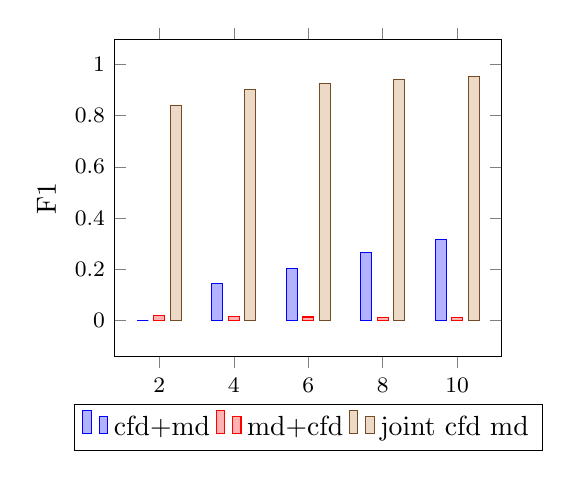
\begin{tikzpicture} \begin{axis}[
ybar,
enlargelimits=0.15,
legend style={at={(0.5,-0.15)}, anchor=north,legend columns=-1},
bar width=4,
ylabel={F1},
symbolic x coords={2,4,6,8,10},
xtick=data,
nodes near coords align={vertical},
]
\addplot coordinates {(2, 0.0) (4, 0.1416) (6, 0.2016) (8, 0.2658) (10, 0.3146)};
\addplot coordinates {(2, 0.0173) (4, 0.0157) (6, 0.012) (8, 0.0087) (10, 0.0088)};
\addplot coordinates {(2, 0.8391) (4, 0.902) (6, 0.9273) (8, 0.9433) (10, 0.9544)};

\legend{cfd+md,md+cfd,joint cfd md}
\end{axis}
\end{tikzpicture}
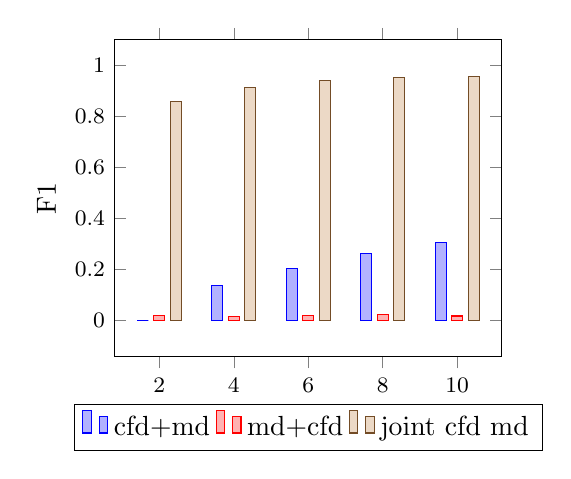
\begin{tikzpicture} \begin{axis}[
ybar,
enlargelimits=0.15,
legend style={at={(0.5,-0.15)}, anchor=north,legend columns=-1},
bar width=4,
ylabel={F1},
symbolic x coords={2,4,6,8,10},
xtick=data,
nodes near coords align={vertical},
]
\addplot coordinates {(2, 0.0) (4, 0.1352) (6, 0.2039) (8, 0.2625) (10, 0.3048)};
\addplot coordinates {(2, 0.0176) (4, 0.0139) (6, 0.0173) (8, 0.0214) (10, 0.016)};
\addplot coordinates {(2, 0.8566) (4, 0.9114) (6, 0.9403) (8, 0.9512) (10, 0.9569)};

\legend{cfd+md,md+cfd,joint cfd md}
\end{axis}
\end{tikzpicture}

\end{document}
